\documentclass[12pt]{article}
%%%%%%%%%%%%%%%%%%%%%
% Header material
%%%%%%%%%%%%%%%%%%%%%

%%%%%%%%%%%%%%%%%%%%%
%  Includes first
%%%%%%%%%%%%%%%%%%%%%
%\usepackage{amsfonts}
%\usepackage{epsf}
\usepackage{placeins}
\usepackage[papersize={8.5in,11in}]{geometry}
\usepackage[pdftex]{graphicx}
\DeclareGraphicsExtensions{.pdf,.png,.jpg}
%\usepackage{draftwatermark}
\usepackage{amsmath}
\usepackage{amsthm}
\usepackage{amssymb}
%\usepackage{txfonts}
\usepackage{textcomp}
%\usepackage{amsthm}
%\usepackage{array}
\usepackage[all]{xy}
\usepackage{fancyhdr}
\usepackage{hyperref}
\usepackage{verbatim}
\usepackage{algorithm}
\usepackage{algorithmic}
\usepackage{color}
\usepackage[usenames,dvipsnames,svgnames,table]{xcolor}
\usepackage{rotating}
\usepackage{wrapfig}
\usepackage{tikz}
\usetikzlibrary{shapes.geometric, arrows}
\usepackage{framed}
\usepackage{multicol}
\usepackage{physics}

\usepackage[utf8]{inputenc}

%%%%%%%%%%%%%%%%%%%%
%  Setup listing environment
%%%%%%%%%%%%%%%%%%%%
\usepackage{listings}
\lstset{language=python,frame=ltrb,framesep=5pt,basicstyle=\small,
 keywordstyle=\ttfamily\color{DarkRed},
%morecomment=[n][\textbf]{In\ [}{]\:},
%morecomment=[n][\textbf]{Out\ [}{]\:},
morecomment=[s][\color{blue}]{In\ [}{]\:},
morecomment=[s][\color{red}]{Out[}{]\:},
identifierstyle=\ttfamily\color{DarkBlue}\bfseries,
commentstyle=\color{OliveGreen},
stringstyle=\ttfamily,
showstringspaces=false,tabsize = 3,
numbers = left}
\usepackage[framemethod=TikZ]{mdframed}
%\usepackage{framed}

\lstdefinelanguage{shell} {
commentstyle = \color{black},
keywordstyle = \color{black},
stringstyle = \color{black},
identifierstyle = \color{black},
morecomment=[s][\color{blue}]{In\ [}{]\:},
morecomment=[s][\color{red}]{Out[}{]\:},
 }

%\definecolor{shadecolor}{gray}{0.9}
\definecolor{shadecolor}{rgb}{0.93,0.95,1.0}


%%%%%%%%%%%%%%%
%  Setup the title region
%%%%%%%%%%%%%%%
\newmdenv [
outerlinewidth = 2,
linecolor = DarkBlue,
roundcorner = 8pt,
leftmargin = 0,
rightmargin = 0,
backgroundcolor = blue!7,
outerlinecolor = blue!70!black,
innertopmargin = \topskip,
splittopskip = \topskip
] {mdtitle}


%%%%%%%%%%%%%
% A few commands
%%%%%%%%%%%%%
\def      \RR             {{\mathbb R}} 
\def      \DS            {\displaystyle} 

%\renewcommand\baselinestretch{1.3}
%% The following block is for narrow margins:
\setlength{\topmargin}{-0.9in}
\setlength{\textheight}{9.50in}
\setlength{\oddsidemargin}{-0.375in}
\setlength{\evensidemargin}{-0.375in}
\setlength{\textwidth}{7.25in}
%% end page descript.
\pagestyle{empty}

\graphicspath{{Resources/}}
\renewcommand{\thesection}{}
\renewcommand{\thesubsection}{}
\hypersetup{
    colorlinks=true,
    linktoc=all,
    citecolor=purple,
    filecolor=green,
    linkcolor=red,
    urlcolor=blue
}

%\makeatletter
%\newcommand{\thickhline}{%
%    \noalign {\ifnum 0=`}\fi \hrule height 1pt
%    \futurelet \reserved@a \@xhline
%}
%\newcolumntype{"}{@{\hskip\tabcolsep\vrule width 1pt\hskip\tabcolsep}}
%\makeatother

\renewcommand{\descriptionlabel}[1]{%
  \hspace\labelsep \upshape\bfseries #1:%
}

%%%%%%%%%%%%%%%%%%%%%%%%%%%
%% Document starts here
%%%%%%%%%%%%%%%%%%%%%%%%%%%

\begin{document}

%%%%%%%%%%%%
% Title
%%%%%%%%%%%%

%\begin{mdtitle}
%\begin{center}
%\begin{Large}
%Notes  \hfill  \scalebox{1.1}{Example Qubit States} \hfill Fall 2016 \\[2mm]
%Quantum Computing \hfill Scott Carda
%\end{Large}
%\end{center}
%\end{mdtitle}
%\vspace*{10mm}

\title{Ternary Emulation Manual}
\date{}
\author{Scott Carda}

\maketitle
\newpage

%%%%%%%%%%%%%%%%%%%%%%%%
%% Table of Contents 
%%%%%%%%%%%%%%%%%%%%%%%%

\tableofcontents
\newpage

%%%%%%%%%%%%
%% Body 
%%%%%%%%%%%%

\section{Introduction} \label{sec:Intro}

\section{Ternary Logic} \label{sec:Logic}

\section{The Emu Emulator} \label{sec:Emu}

Heptavigesimal Numbering System

\section{Instruction Format} \label{sec:Format}
               
\begin{figure}[h!]
    \centering
    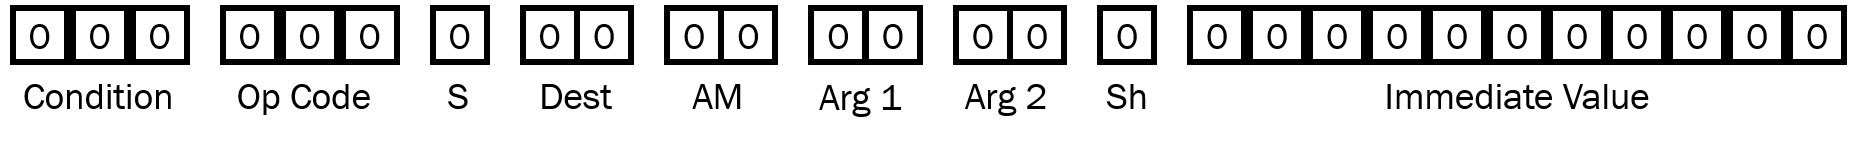
\includegraphics[width=\linewidth]{Resources/Instruciton_Format.png}
    \caption
    {
        27-trit Instruciton Format
    } \label{fig:Instruction Format}
\end{figure}

\begin{description}
\item[Condition] The 3-trit condition code the machine uses to determine whether the instruction is executed.
\item[Op Code] The 3-trit code that indicates which operation is performed with this instruction.
\item[S] The instruction's flag mode. The jump operation has unique behavior associated with this.
\item[Dest] The 2-trit indicator for the destination register.
\item[AM] The instruction's 2-trit address mode.
\item[Arg 1] The 2-trit indicator for the register to be used as the first argument to the operation.
\item[Arg 2] The 2-trit indicator for the register to be used as the second argument to the operation.
\item[Sh] The instruction's shift mode. Indicates which shift operation is performed on Arg 2.
\item[Immediate Value] This 11-trit field is reserved for embedding numerical values in the instruction.
\end{description}
    
\section{Conditions} \label{sec:Conditions}

The Current Program Status Register or CPSR is a special 3-trit register that keeps track of several flags. There are three flag, one associated with each of the three trits in the register. The most significant trit is the \textbf{S} flag, which indicates the sign of the result of an operation. \hyperref[tab:S Values]{Table \ref{tab:S Values}} shows the meaning of the values for the \textbf{S} flag. The middle of the three trits is the \textbf{C} flag, which contains the value of any unsigned overflow resulting from an operation. The least significant trit is the \textbf{V} flag, which contains the value of any signed overflow resulting from an operation.

\begin{table}[h!]
    \centering
    %\caption{\textbf{S} Flag Values}
    \caption{}
    \label{tab:S Values}
    \begin{tabular}{|c|l|} 
        \hline
        %\textbf{S} & Meaning \\ [0.5ex] \hline
        \textbf{S} & Meaning \\ \hline
        0 & Result was Positive \\ \hline
        1 & Result was Zero \\ \hline
        %2 & Result was Negative \\ [1ex] \hline
        2 & Result was Negative \\ \hline
    \end{tabular}
\end{table}

Instruction are conditionally executed based on the values of these flag. Common conditions have been abstracted from these flag and made available to the system. Each condition is assigned a 3-trit code for use in the most significant field of an instruction. If the condition is false, the rest of the instruction is ignored, and the machine will move on to the next instruction in its RAM without executing the encoded operation. The conditions available to the system are found in \hyperref[tab:Conditions]{Table \ref{tab:Conditions}}.

\begin{table}[h!]
    \centering
    \caption{}
    \label{tab:Conditions}
    \begin{tabular}{|c|l|c|} 
        \hline
        \textbf{Condition Code} & Meaning & Flags \\ \hline
        
        000 & Always & Always \\ \hline
        001 & Equal & \textbf{S} = 1 \\ \hline
        002 & Carry Clear & \textbf{C} = 0 \\ \hline
        010 & Negative & \textbf{S} = 2 \\ \hline
        011 & Overflow Clear & \textbf{V} = 0 \\ \hline
        012 & Unsigned Lower/Equal & \textbf{C} = 0 \textbf{OR} \textbf{S} = 1 \\ \hline
        020 & Less Than & IS\_T(\textbf{S}) = IS\_F(\textbf{V}) \\ \hline
        021 & Less Than or Equal To & \textbf{S} = 1 \textbf{OR} IS\_T(\textbf{S}) = IS\_F(\textbf{V}) \\ \hline
    
        022-200 & \textit{bad condition code} & \textit{bad condition code} \\ \hline
    
        201 & Greater Than & \textbf{S} $\neq$ 1 \textbf{AND} IS\_T(\textbf{S}) $\neq$ IS\_F(\textbf{V}) \\ \hline
        202 & Greater Than or Equal To & IS\_T(\textbf{S}) $\neq$ IS\_F(\textbf{V}) \\ \hline
        210 & Unsigned Higher & \textbf{C} $\neq$ 0 \textbf{AND} \textbf{S} $\neq$ 1 \\ \hline
        211 & Overflow Set & \textbf{V} $\neq$ 0 \\ \hline
        212 & Positive & \textbf{S} $\neq$ 2 \\ \hline
        220 & Carry Set & \textbf{C} $\neq$ 0 \\ \hline
        221 & Not Equal & \textbf{S} $\neq$ 1 \\ \hline
        222 & Never & Never \\ \hline
    \end{tabular}
\end{table}

\section{Operations} \label{sec:Operations}

\section{Flag Mode} \label{sec:Flag Mode}

\section{Address Mode} \label{sec:Address Mode}

\section{Shift Mode} \label{sec:Shift Mode}

\section{Immediate Value} \label{sec:Immediate Value}

\section{Raw} \label{sec:Raw}
    
27 trits
  xxx   xxx  x  xx  xx  xx   xx   x  xx-xxxxxxxxx
 cond opcode s arg1 AM arg2 arg3 shf  val 
               dest    opr1 opr2
    
Conditions:
    
    000:    Always
    001:    Equal ( S flag = 1 )
    002:    Carry Clear ( C flag = 0 )
    010:    Negative ( S flag = 0 )
    011:    Overflow Clear ( V flag = 0 )
    012:    Unsigned Lower ( C flag = 0, OR S flag = 1 )
    020:    $<$ ( IS\_F(S flag) = IS\_F(V flag) )    
    021:    $<=$ ( S flag = 1 OR IS\_F(S flag) = IS\_F(V flag) )
    
    022-200:   $<$bad$>$
    
    201:    $>$ ( S flag = 1 AND IS\_F(S flag) != IS\_F(V flag) )
    202:    $>=$ ( IS\_F(S flag) != IS\_F(V flag) )
    210:    Unsigned Higher ( C flag != 0 AND S flag != 1 )
    211:    Overflow Set ( V flag != 0 )
    212:    Positive ( S flag != 0 ) - maybe: ( S flag = 2 )
    220:    Carry Set ( C flag != 0 )
    221:    Not Equal ( S flag != 1 )
    222:    Never
        
Shift Values:

    0: LSR
    1: ASR
    2: LSL
        
Address Modes (AM):
    
    00:     Immediate -         Data found in Instruction ( val ) - Ignore opr2 and shf
        MOV     r0, $\#$3          000 022 0 00 00 xx xx x 00-000000010 = 00002200000xxxxx00000000010
        ADD     r0, r1, $\#$3      000 020 0 00 00 01 xx x 00-000000010 = 0000200000001xxx00000000010
        
    01:     Reg Direct -        Register of Data found in Instruction ( opr2 ) - Ignore shf and val
        MOV     r0, r1          000 022 0 00 01 xx 01 x xx-xxxxxxxxx = 00002200001xx01xxxxxxxxxxxx
        
    02:     Reg Dir Scalled -   Register of Data and Scale found in Instruction ( val )
        ADD     r0, r1, r2, LSL $\#$15
                                000 020 0 00 02 01 02 2 00-000000120 = 000020000020102200000000120
    
    10:     $<$bad$>$
        
    11:     Addressed -         Address of Data found in Instruction ( val ) - Ignore opr1, opr2, and shf
        LDR     r0, [$\#$$<$address$>$]
                                000 010 0 00 11 xx xx x ss-$<$address$>$ = 00001000011xxxxxss$<$address$>$
        
    12:     Reg Indirect -      Address of Data stored in Register found in Instruction ( opr1 ) - Ignore opr2, shf, and val
        LDR     r0, [r1]        000 010 0 00 12 01 xx x xx-xxxxxxxxx = 0000100001201xxxxxxxxxxxxxx
        
    20:     -w/ Imm Offset -    Reg Indirect Address plus Offset found in Instruction ( Reg: opr1, Off: val ) - Ignore opr2 and shf
        LDR     r0, [r1, $\#$3]    000 010 0 00 20 01 xx x 00-000000010 = 0000100002001xxx00000000010
        
    21:     -w/ Dir Offset -    Reg Indirect Address plus Offset found in Reg in Instruction ( Reg: opr1, Off: opr2 ) - Ignore shf and val
        LDR     r0, [r1, r2]    000 010 0 00 21 01 02 x xx-xxxxxxxxx = 000010000210102xxxxxxxxxxxx
                                
    22:     -w/ Scaled Offset - Reg Indirect Address plus Scaled Offset found in Reg in Instruction, Scale is found in Instruction
                                ( Reg: opr1, Off: opr2, Scale: val )
        LDR     r0, [r1, r2, LSL $\#$1]
                                000 010 0 00 22 01 02 2 00-000000001 = 000010000220102200000000001
    
Opcodes:

    (@) 000: HALT
    (A) 001: NO\_OP
    (B) 002: CLEAR

    (C) 010: LOAD
    (D) 011: STORE
    (E) 012: EXCHANGE

    (F) 020: ADD
    (G) 021: SUB
    (H) 022: MOVE

    (I) 100: AND
    (J) 101: OR
    (K) 102: XOR

    (L) 110: F\_NOT
    (M) 111: N\_NOT
    (N) 112: T\_NOT

    (O) 120: ISF
    (P) 121: ISN
    (Q) 122: IST

    (R) 200: LSR
    (S) 201: ASR
    (T) 202: LSL

    (U) 210: SHIFT\_M
    (V) 211: SHIFT\_P
    (W) 212: $<$bad$>$

    (X) 220: JUMP
    (Y) 221: $<$bad$>$
    (Z) 222: $<$bad$>$

%\include{Sections/Bloch_Sphere}

%\include{Sections/Mathy}

%\include{Sections/Transformation_Definitions}

%\include{Sections/Examples}

\end{document}
